%!TEX root = ./main.tex

\section{The model}

\begin{frame}{The model}

\alert{Goal}: given a set of $n$ data with $p$ variables, simultaneously infer the conditional dependence structure of such variables and their clustering.

\pause

\alert{Constraint}: the partition must respect the original order of the variables.
\pause
\begin{align*}
    \bm{y}_1, \ldots, \bm{y}_n \mid \bm{K} & \iid \mathcal{N}_p(\mathbf{0}, \bm{K}^{-1} ) \\
    \bm{K} \mid G & \sim \GWish(b, D)\\
    P((i,j)&\in E\mid \bm{z},Q) = Q_{z_{i} z_{j}},\,\text{independent}\\
        Q_{rs} \mid \bm{z} &\ind \Beta(\alpha,\beta), 1\leq r\leq s\leq M\\
    \rho & \sim f_{\rho} \left(\rho\right)
\end{align*}

Notation for the partition: $\rho$ vector of cardinalities, $\bm{z}$ vector of groups memberships.

The prior for the \alert{partition} $f_{\rho}(\rho)$ is (5) from \cite{martinezNonparametricChangePoint2014}.

\end{frame}

\begin{frame}

$Q$ is marginalized out.
\pause

The prior for the \alert{graph} given the vector of group memberships is
\[
    P(G\mid \bm{z})
    =
    \prod_{u=1}^{M}\prod_{v=u}^{M}
    \frac{B(\alpha + S_{uv}, \beta+ S^{\star}_{uv})}{B(\alpha,\beta)}
\]
where 
\begin{itemize}
    \item $S_{uv}$ is the sum of the edges between group $u$ and $v$.
    \item $S^{\star}_{uv}$ is the sum of the ``non-edges'', namely $S^{\star}_{uv} = T_{uv} - S_{uv}$ and $T_{uv}$ is the total number of possible edges.
\end{itemize}
\pause


\end{frame}

\section{The sampling strategy}

\subsection{Overview of the sampling strategy}

\begin{frame}{Block Gibbs Sampler}
    Conditional distributions for our model:
    \begin{table}[tb]
        \centering
        \begin{tabular}{ll}
        \toprule
        Graph and Precision & $\small P(\bm{K},G \mid \bm{Y},\bm{z}) \propto P(\bm{Y} \mid \bm{K})P(\bm{K} \mid {G}) P(G \mid \bm{z})$ \\
        \hline
        Random Partition & $\small P(\bm{z} \mid \bm{Y},\bm{K},G) \propto P(\bm{Y} \mid \bm{K})P(\bm{K} \mid {G})P(G \mid \bm{z})P(\bm{z}) \propto P(G \mid \bm{z})P(\bm{z}) $ \\
        \bottomrule
        \end{tabular}
    \end{table}

    \pause 

    We implement a Block Gibbs-Sampler strategy:
    \begin{enumerate}
        \item \alert{Sampling Graph and Precision Matrix}\\
        $G$ and $\bm{K}$ - given $\bm{z}$ - are sampled using a modified version of a Birth-and-Death chain (\cite{mohammadiBayesianStructureLearning2015a}), changing one link at a time.
        \item \alert{Sampling the Random Partition}\\
        Conditionally on $G$, we can sample $\bm{z}$ through an adaptive split and merge\vphantom{changepoint} sampler.
    \end{enumerate}
\end{frame}

\subsection{Updating the graph}

\begin{frame}{Birth and death algorithm for updating the graph}

    \texttt{BDGraph} is an algorithm that follows a Birth-and-Death approach to decide whether to \alert{add} a new edge to the graph or \alert{delete} an already existing one.

    \pause
    
    % https://people.inf.ethz.ch/markusp/teaching/guides/guide-tables.pdf
    \begin{table}[tb]
        \centering
        \begin{tabular}{lcc}
        \toprule
        & Target distribution & B/D rates \\
        \hline
        \textbf{Before} & $P(G,\bm{K} \mid \bm{Y}) \propto \mathcal{L}(\bm{Y} \mid \bm{K})\mathcal{L} (\bm{K} \mid {G})P(G)$ & $\cfrac{P(G')}{P(G)}$ \\
        \textbf{After}  & $P(G,\bm{K} \mid \bm{Y}, \textcolor{sleekRed}{\bm{z}}) \propto \mathcal{L}(\bm{Y} \mid \bm{K})\mathcal{L}(\bm{K} \mid {G})P(G \mid \textcolor{sleekRed}{\bm{z}})$ & $\cfrac{P(G' \mid \textcolor{sleekRed}{\bm{z}})}{P(G \mid \textcolor{sleekRed}{\bm{z}})}$ \\
        \bottomrule
        \end{tabular}
    \end{table}
    where $G' = G^{\pm e}$ and $e$ is an edge.
    \pause
    \[
        \text{Birth rate} \propto \frac{P(G^{+ e}\mid \bm{z})}{P(G\mid \bm{z})} = \frac{S_{uv} + \alpha}{S^{\star}_{uv} + \beta}
        \quad
        \text{Death rate} \propto \frac{P(G^{- e}\mid \bm{z})}{P(G\mid \bm{z})} = \frac{S^{\star}_{uv} + \beta}{S_{uv} + \alpha}
    \]
    
\end{frame}

\subsection{Updating the partition}

\begin{frame}{General steps for updating the partition}
    
    We perform an adaptive \alert{split and merge}.

    \fg{0.45}{update_partition_splitmerge.pdf}
    \begin{enumerate}
        \item With probability $\alpha_{\text{split}}$, usually $0.5$, choose an \alert{split move}, otherwise a \alert{merge move}. Unless we are forced by extreme cases.
        \begin{enumerate}
            \item Propose a new partition by splitting one group into two or merging two adjacent.
            \item Accept or reject using\vphantom{un banale} Metropolis Hastings. The target is:
            $f(\rho \mid G) \approx f_G(G \mid \rho) f_{\rho}(\rho)$
            \[
                \alpha_{\text{accept}} = \min
                \bigg\{1,
                \overbrace{
                \underbrace{\frac{f_G\left(G \mid \rho'\right)}{f_G(G \mid \rho)}}_{\substack{\text{graph}\\\text{ratio}}}
                \underbrace{\frac{f_\rho\left(\rho'\right)}{f_\rho(\rho)}}_{\substack{\text{partition}\\\text{ratio}}}
                }^{\text{target ratio}}
                \underbrace{\frac{Q(\rho',\rho)}{Q(\rho,\rho')}}_{\substack{\text{proposal}\\\text{ratio}}}
                \bigg\}
            \]
        \end{enumerate}
        
    \end{enumerate}

\end{frame}

\begin{frame}{Shuffle move}
    \begin{enumerate}
        \item[2.] To improve the mixing of the chain we also perform a \alert{shuffle move}.
            \begin{enumerate}
                \item[2.1] Propose a new partition by moving some nodes from a group to an adjacent one.
                \item[2.2] Accept or reject using Metropolis Hastings.
            \end{enumerate}
    \end{enumerate}

    \fg{0.4}{update_partition_shuffle.pdf}
\end{frame}

\begin{frame}{Partition ratio}

We introduce $\bm{a}^{(t)}$ and $\bm{d}^{(t)}$, two $(p-1)$-dimensional vectors of \alert{weights} to choose the node where to perform the split or the merge. They are unnormalized discrete densities.

\pause

Suppose a split move.

\pause

At each iteration, \alert{draw} node $i$ with probability proportional to $a_{i}^{(t)}$.

\pause

Denoting by $a^{\star} = \sum_{j\in \{\text{admissible split nodes}\}}{a_{j}^{(t)}}$ and $d^{\star} = \sum_{j\in \{\text{admissible merge nodes}\}}{d_{j}^{(t)}}$

\pause

\[
    \frac{Q(\rho',\rho)}{Q(\rho,\rho')}
    =
    \frac{P(\text{choose merge})}{P(\text{choose split})}
    \cdot 
    \frac{P(\text{merge at node $i$})}{P(\text{split at node $i$})}
    =
    \frac{1-\alpha_{\text{split}}}{\alpha_{\text{split}}}
    \cdot
    \frac{\frac{d_{i}^{(t)}}{d^{\star}+d_{i}^{(t)}}}{\frac{a_{i}^{(t)}}{a^{\star}}}
\]
The extreme cases ``every node belonging to the same group'' and ``every node has its own group'' are dealt with separately.

\end{frame}

\begin{frame}{Adaptive step}
    The two weights vectors $\bm{a}^{(t)}$ and $\bm{d}^{(t)}$ are updated at each iteration $t$ as in \cite{bensonAdaptiveMCMCMultiple2018} using the following 
    \textbf{adaptation scheme}.

    \begin{itemize}
        \item If a \alert{split} move at node $i$ has been accepted, then update:
		\[
		\log (a_i^{(t+1)})=\log (a_i^{(t)})+\frac{h}{t/p}(\alpha_{\text{split}}-\alpha_{\text{target}}) .
		\]
        \item If a \alert{merge} move at node $i$ has been accepted, then update:
		\[
		\log (d_i^{(t+1)})=\log (d_i^{(t)})+\frac{h}{t/p}(\alpha_{\text{merge}}-\alpha_{\text{target}}) .
		\]
        \end{itemize}
Where $h>0$ is the initial adaptation, $t/p$ are the iterations $(t)$ per number of nodes $(p)$, $\alpha_{\text{target}}$ is the target MH acceptance rate and $\alpha_{\text{merge}} = 1 - \alpha_{\text{split}}$.

\end{frame}

\section{Next steps}

\begin{frame}{Next steps}

The first draft of the code is completed.

Next things to do:
    \begin{itemize}
        \item debugging the code
        \item run simulations
        \item perform posterior analysis
    \end{itemize}

\end{frame}

\begin{frame}{Main references}
    % GGM
    \nocite{colombiLearningBlockStructured2022a}
    \nocite{mohammadiBayesianStructureLearning2015a}
    % SBM
    \nocite{legramantiExtendedStochasticBlock2022}
    % Changepoint
    \nocite{bensonAdaptiveMCMCMultiple2018}
    \nocite{martinezNonparametricChangePoint2014}
    
    \printbibliography
    \renewcommand*{\bibfont}{\small}
\end{frame}

\begin{frame}[plain]
    % Add background to content page
    \AddToShipoutPictureFG*{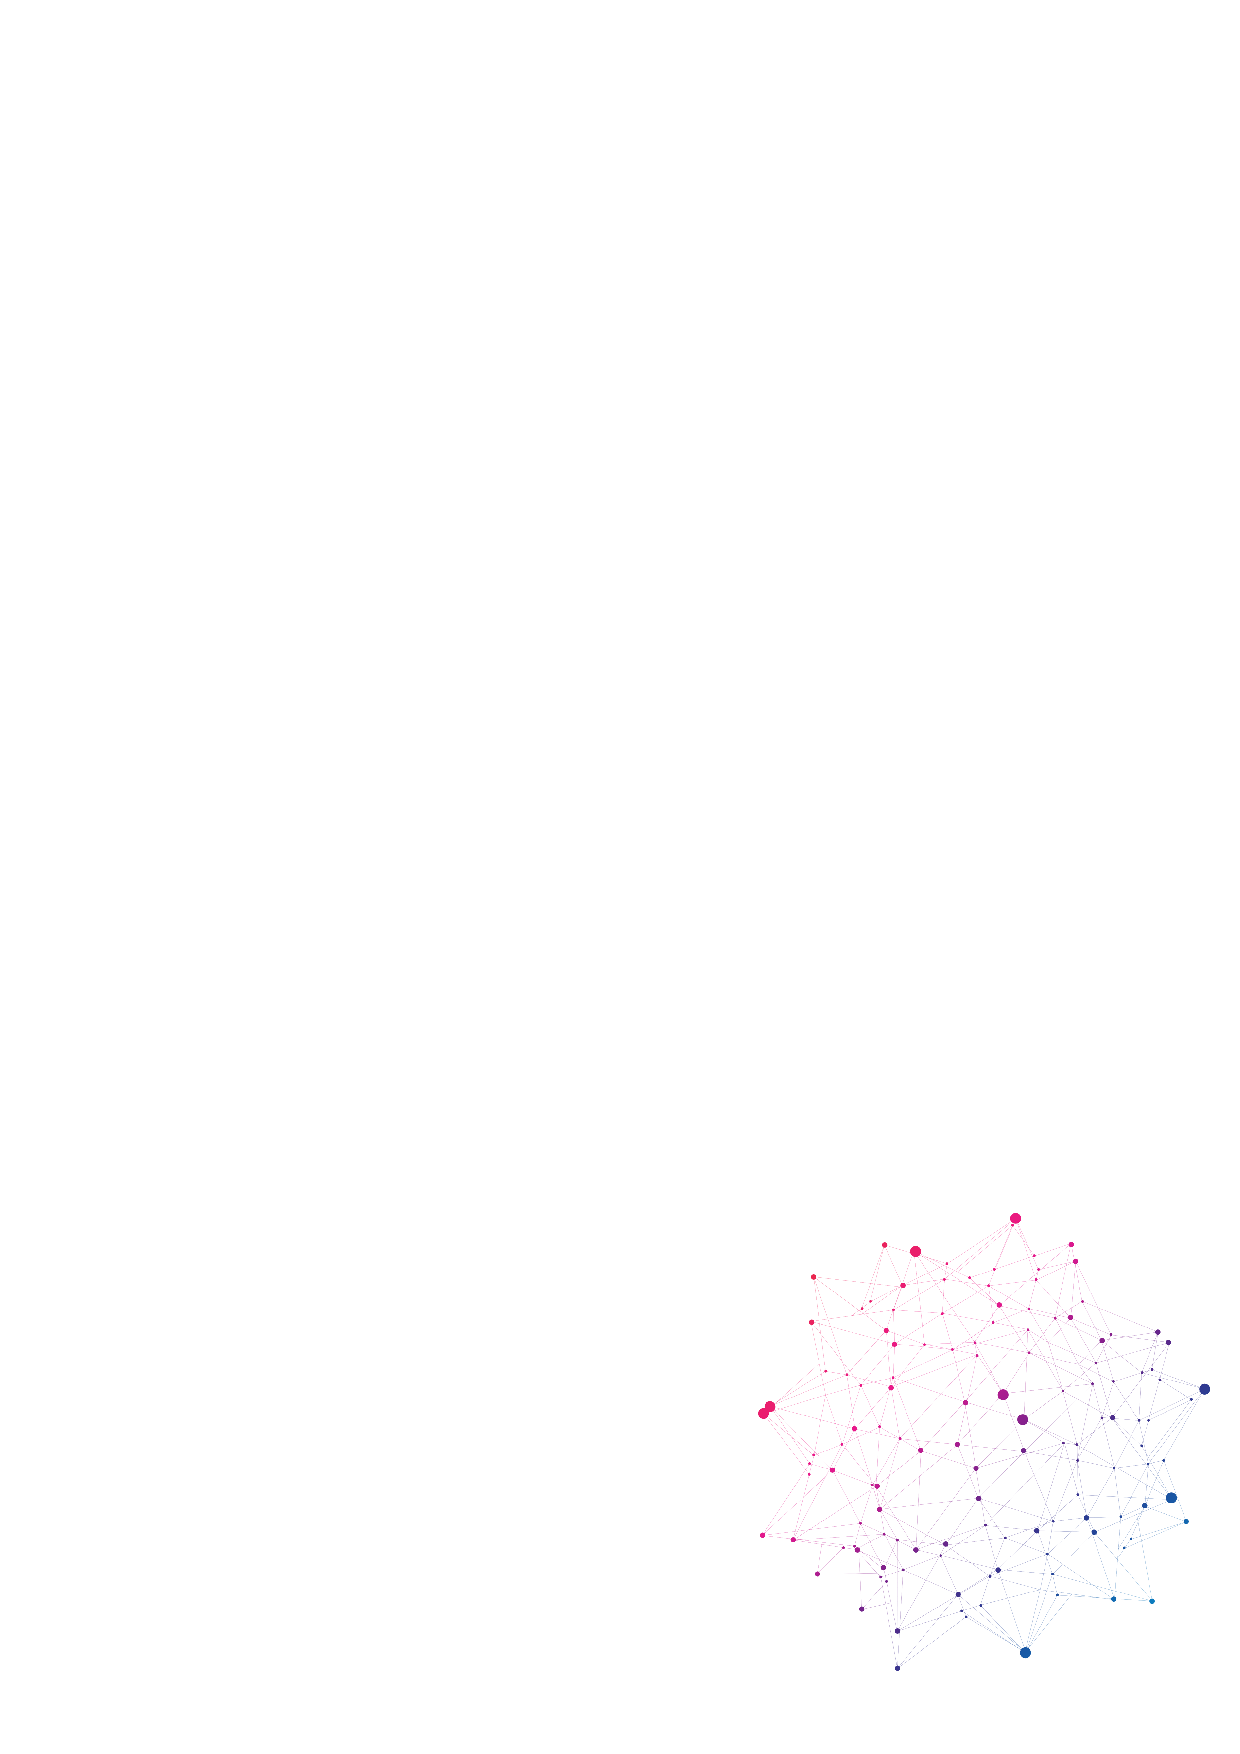
\includegraphics[width=\paperwidth]{Images/background.pdf}}
    \vspace*{1.2cm}
    \hspace*{1cm}{\Large Thank you!}\\
    \vspace*{0.6cm}
    \hspace*{1cm}{\Huge \alert{Any questions?}}
\end{frame}

\section*{Extra}

\begin{frame}{Partition ratio}

As a prior, we use an EPPF induced by the \alert{two-parameter Poisson-Dirichlet} process (Pitman-Yor process) from \cite{martinezNonparametricChangePoint2014}.

Let $M$ and $p$ be the number of groups and nodes, respectively, and $n_{j},j=1,\ldots,M$ the cardinalities of the groups, $\theta$ and $\sigma$ are parameters.
\begin{equation*}
    P(\rho = \{n_1, \ldots, n_M\})
    =
    \begin{cases}
        \frac{p!}{M!} \frac{ \prod_{i=1}^{M-1}{(\theta +i\sigma)} }{(\theta+1)_{(p-1)\uparrow}} \prod_{j=1}^{M}{\frac{(1-\sigma)_{(n_{j}-1)\uparrow}}{n_{j\uparrow}} }, & \rho \text{ admissible} \\
        0, & \rho \text{ not admissible.}
    \end{cases}
\end{equation*}

Hence, in the split case, after simplifying common factors, the \alert{partition ratio} is:

\begin{equation*}
    \frac{f_{\rho}(\rho')}{f_{\rho}(\rho)}
    =
    \frac{1}{M}(\theta+M\sigma)\frac{(1-\sigma)_{(n_{s}'-1)\uparrow}(1-\sigma)_{(n_{s}'+1)\uparrow}}{(1-\sigma)_{(n_{s}-1)\uparrow}}\frac{n_{s}!}{n'_{s}!n'_{s+1}!}
\end{equation*}

\end{frame}

\begin{frame}{Graph ratio}

Suppose a split move.

The \alert{graph ratio}, after simplifying common factors, is:
{
    \footnotesize
    \begin{align*}
        & \frac{f_G(G \mid \rho^\prime)}{f_G(G \mid \rho)}=\left(\frac{1}{B(\alpha, \beta)}\right)^{M+1} \times \\
        & \frac{ \prod_{l=1}^{S-1} f_B(C_l^\prime, C_S^\prime) f_B(C_l^\prime, C_{S+1}^\prime) \cdot \prod_{m=S+2}^{M+1} f_B(C_S^\prime, C_m^\prime) f_B(C_{S+1}^\prime, C_m^\prime) \cdot f_B(C_S^\prime, C_{S+1}^\prime) f_B(C_S^\prime, C_S^\prime) f_B(C_{S+1}^\prime, C_{S+1}^\prime)}{\prod_{l=1}^{S-1} f_B(C_l, C_S) \prod_{m=S+1}^M f_B(C_S, C_m) \cdot f_B(C_S, C_S)}
    \end{align*}
}

where

\[
    f_B(C_u, C_v) = B(\alpha+S_{uv},\beta+S^{\star}_{uv})
\]

\end{frame}
